%%----------------------------------------------------------------------------------------
%	PACKAGES AND THEMES
%----------------------------------------------------------------------------------------
\PassOptionsToPackage{table}{xcolor}
\documentclass[aspectratio=169,xcolor=dvipsnames,svgnames,x11names,fleqn]{beamer}
% \documentclass[aspectratio=169,xcolor=dvipsnames,fleqn]{beamer}

\usetheme{RedVelvet}

\usefonttheme[onlymath]{serif}
\newcommand{\showanswers}{yes}
\usepackage{pifont} % For checkmarks and crosses

\usepackage{setspace}
\usepackage{xspace}
\usepackage{amsmath}
\usepackage{amssymb}
\usepackage{amsfonts}
\usepackage{color}
\usepackage{physics}
% \usepackage{mathbb}
\usepackage{rahul_math}
\usepackage{bigints}

\usepackage[utf8]{inputenc}
\usepackage[ruled,vlined]{algorithm2e}
\usepackage{amsmath}
\usepackage{amsfonts}

\usepackage{graphicx} % Allows including images
\usepackage{booktabs} % Allows the use of \toprule, \midrule and \bottomrule in tables
\usepackage{tikz,pgfplots}
\usepackage{mathtools}
\usepackage{subfigure}
\usetikzlibrary{arrows}
\usepackage{minted}
\definecolor{LightGray}{gray}{0.9}
\definecolor{cream}{rgb}{0.92, 0.9, 0.55}
\definecolor{lightblue}{rgb}{0.68, 0.85, 0.9}


\usepackage{xcolor-material}
\usetikzlibrary{fit}
\usetikzlibrary{matrix}
\tikzset{%
apple/.pic={
    \fill [MaterialBrown] (-1/8,0)  arc (180:120:1 and 3/2) coordinate [pos=3/5] (@)-- ++(1/6,-1/7)  arc (120:180:5/4 and 3/2) -- cycle;
    \fill [MaterialLightGreen500] (0,-9/10)  .. controls ++(180:1/8) and ++(  0:1/4) .. (-1/3,  -1) .. controls ++(180:1/3) and ++(270:1/2) .. (  -1,   0) .. controls ++( 90:1/3) and ++(180:1/3) .. (-1/2, 3/4) .. controls ++(  0:1/8) and ++(135:1/8) .. (   0, 4/7)
    }
    }

\newcommand{\leftdoublequote}{\textcolor{blue}{\scalebox{3}{``}}}

\newcommand{\rightdoublequote}{\textcolor{blue}{\scalebox{3}{''}}}


\usepackage{textcomp}
\usepackage{fontawesome}
\usepackage{tikz,pgfplots}
\usetikzlibrary{shapes.callouts}
\usetikzlibrary{arrows}
\usetikzlibrary{shapes.geometric, positioning}
\usetikzlibrary{matrix,positioning,decorations.pathreplacing,calc}
\usepackage{tikz-dependency}

\pgfplotsset{compat=1.8} % or newest version

\usetikzlibrary{positioning}


\usepackage{bm}
\usepackage{relsize}

\tcbuselibrary{skins, hooks}

\tikzset{basic/.style={draw,fill=MediumBlue!20,text width=1em,text badly centered}}
\tikzset{input/.style={basic,circle}}
\tikzset{weights/.style={basic,rectangle}}
\tikzset{functions/.style={basic,circle,fill=MediumBlue!10}}



\usepackage{listofitems} % for \readlist to create arrays
\tikzstyle{mynode}=[thick,draw=MediumBlue,fill=MediumBlue!20,circle,minimum size=22]


\usepackage{overpic}

%----------------------------------------------------------------------------------------
%	TITLE PAGE
%----------------------------------------------------------------------------------------

\usepackage{tikz-qtree,tikz-qtree-compat}
\usetikzlibrary{tikzmark}
\usetikzlibrary{calc}

\usetikzlibrary{fit}
\tikzset{%
apple/.pic={
    \fill [MaterialBrown] (-1/8,0)  arc (180:120:1 and 3/2) coordinate [pos=3/5] (@)-- ++(1/6,-1/7)  arc (120:180:5/4 and 3/2) -- cycle;
    \fill [MaterialLightGreen500] (0,-9/10)  .. controls ++(180:1/8) and ++(  0:1/4) .. (-1/3,  -1) .. controls ++(180:1/3) and ++(270:1/2) .. (  -1,   0) .. controls ++( 90:1/3) and ++(180:1/3) .. (-1/2, 3/4) .. controls ++(  0:1/8) and ++(135:1/8) .. (   0, 4/7)
}
}
\usepackage{tikz-qtree,tikz-qtree-compat}
\usetikzlibrary{tikzmark}
\usetikzlibrary{calc}

\usetikzlibrary{positioning}
\newcommand{\vect}[1]{\mathbf{#1}}
% Define styles
\tikzset{
    box/.style={
        rectangle,
        draw=black,
        fill=blue!20,
        text width=2.2cm,
        text centered,
        minimum height=0.8cm,
        font=\small
    },
    arrow/.style={
        ->,
        >=Stealth,
        line width=1.5pt,
        draw=black
    }
}


\usepackage{bm}
\usepackage{relsize}



\tikzset{basic/.style={draw,fill=MediumBlue!20,text width=1em,text badly centered}}
\tikzset{input/.style={basic,circle}}
\tikzset{weights/.style={basic,rectangle}}
\tikzset{functions/.style={basic,circle,fill=MediumBlue!10}}
\usetikzlibrary{arrows.meta, bending}
\usetikzlibrary{shapes.geometric, arrows.meta, positioning, fit, backgrounds}

\usepackage{listofitems} % for \readlist to create arrays
\tikzstyle{mynode}=[thick,draw=MediumBlue,fill=MediumBlue!20,circle,minimum size=22]


\newmdenv[
backgroundcolor=androidYellowLight,
linecolor=androidYellow,
linewidth=0.5pt,
roundcorner=10pt,
skipabove=\baselineskip,
skipbelow=\baselineskip
]{MintedFrame}

% Set minted options
\setminted{
fontsize=\footnotesize,
breaklines=true,
autogobble,
linenos,
frame=none
}


\title[CPE 487/587: Deep Learning]{CPE 486/586: Deep Learning for Engineering Applications} % The short title appears at the bottom of every slide, the full title is only on the title page
\subtitle{12 Neural Ordinary Differential Equations}

\author[Rahul Bhadani] {{\Large \textbf{Rahul Bhadani}}}

\institute[UAH] % Your institution as it will appear on the bottom of every slide, maybe shorthand to save space
{
    Electrical \& Computer Engineering,  The University of Alabama in Huntsville
}
\date

% \titlegraphic{
%    \includegraphics[width=0.4\linewidth]{figures/UAH_primary.png}
% }

\newcommand{\N}{\mathcal{N}}


\begin{document}

%-------------------------------------------------
\begin{frame}
    \titlepage
\end{frame}

%-------------------------------------------------
\begin{frame}{Outline}
    \backgroundtableofcontents
\end{frame}

%------------------------------------------------
\section{Motivation}
%------------------------------------------------

\begin{frame}{Ordinary Differential Equations}


\scriptsize

\begin{columns}
\column{0.62\textwidth}
\begin{tblockFrost}{Initial Value Problems}

  \begin{align*}
    \frac{dx(t)}{dt} = f(x(t), t, \theta); \quad x(t_0) \text{ is given}; \quad x(t_1) = \;?
  \end{align*}

  \begin{itemize}
    \item $x$ is a variable we are interested in,
    \item $t$ is (typically) time,
    \item $f$ is a function of $x$ and $t$; it is the differential,
    \item $\theta$ parameterizes $f$ (optionally).
  \end{itemize}

\end{tblockFrost}
\begin{alertblock}{}
  \begin{center}
    \fbox{Many physical processes follow this template!}
  \end{center}\end{alertblock}
\column{0.34\textwidth}

  \textbf{Solution:}
  \begin{align*}
    x(t_1) = x(t_0) + \int_{t_0}^{t_1} f(x(t), t, \theta)\, dt
  \end{align*}
 
  \begin{block}{Example}
    \begin{align*}
      \frac{dx}{dt} &= 2t;\quad x(0) = 2;\quad x(1) = \;?\\
      \Rightarrow x(1) &= x(0) + \int_0^1 2t\, dt\\
                       &= x(0) + \bigl(t^2\big|_{t=1} - t^2\big|_{t=0}\bigr)\\
                       &= 2 + 1^2 - 0^2 = 3
    \end{align*}
  \end{block}

\end{columns}

\end{frame}


\begin{frame}{Ordinary Differential Equations (ODEs)}

\scriptsize

  \begin{align*}
    x(t_1) = x(t_0) + \boxed{\int_{t_0}^{t_1} f(x(t), t, \theta)\, dt}
    \quad \longrightarrow \text{ What if this cannot be analytically integrated?}
  \end{align*}
 
  \begin{block}{Example}
    \begin{align*}
      \frac{dx}{dt} &= 2xt;\quad x(0) = 3\\
      \Rightarrow \int \frac{1}{2x}\, dx &= \int t\, dt\\
      \Rightarrow \tfrac{1}{2}\log x &= \tfrac{1}{2}t^2 + c_0\\
      \Rightarrow x(t) &= ce^{t^2},\quad x(0) = 3 \Rightarrow c = 2\\
      \therefore x(t) &= 2e^{t^2} \Rightarrow x(1) = 5.436
    \end{align*}
  \end{block}
\end{frame}
 
 
 \begin{frame}{Ordinary Differential Equations (ODEs)}


  \begin{align*}
    x(t_1) = x(t_0) + \int_{t_0}^{t_1} f(x(t), t, \theta)\, dt
  \end{align*}
 
  \begin{block}{Approximations to $\int_{t_0}^{t_1} f(x(t),t,\theta)\,dt$\;  i.e.\ \textbf{Numerical Integration}}
    \begin{itemize}
      \item Euler method
      \item Runge-Kutta methods
      \item \ldots
    \end{itemize}
  \end{block}
\end{frame}

\begin{frame}{Ordinary Differential Equations (ODEs)}
  \textbf{Initial value problem:}
  \begin{align*}
    \frac{dx(t)}{dt} = f(x(t), t, \theta); \quad x(t_0) \text{ is given}; \quad x(t_1) = \;?
  \end{align*}
 
  \textbf{Solution:}
  \begin{align*}
    x(t_1) = x(t_0) + \int_{t_0}^{t_1} f(x(t), t, \theta)\, dt
  \end{align*}
 
  \begin{block}{\textbf{1st-order Runge-Kutta / Euler's method}}
    \begin{align*}
      t_{n+1} &= t_n + h \quad \longrightarrow \text{ Step size } h\\
      x(t_{n+1}) &= x(t_n) + h\,f(x(t_n), t_n) \quad \longrightarrow \text{ Update using derivative } f
    \end{align*}
  \end{block}
 
  \begin{center}
    \textit{Step size matters!}
  \end{center}
\end{frame}
 
 
% ------------------------------------------------------------
\begin{frame}{Ordinary Differential Equations (ODEs) -- Euler Example}
  \textbf{1st-order Runge-Kutta / Euler's method:}
  \begin{align*}
    t_{n+1} &= t_n + h\\
    x(t_{n+1}) &= x(t_n) + h\,f(x(t_n), t_n)
  \end{align*}
 
  \begin{block}{Example: $\frac{dx}{dt} = f(x,t) = 2xt$; $x(0)=3$; $x(1)=?$\quad (True: $x(1) \approx 5.436$)}
    \small
    \begin{align*}
      h &= 0.25\\
      x(0.25) &= x(0) + 0.25 \cdot f(x(0),0) = 3 + 0.25\cdot(2\cdot3\cdot0) = 3\\
      x(0.5)  &= x(0.25) + 0.25\cdot f(x(0.25),0.25) = 3 + 0.25\cdot(2\cdot3\cdot0.25) = 3.375\\
      x(0.75) &= x(0.5) + 0.25\cdot f(x(0.5),0.5) = 3.375 + 0.25\cdot(2\cdot3.375\cdot0.5) = 4.21875\\
      x(1)    &= x(0.75) + 0.25\cdot f(x(0.75),0.75)\\
              &= 4.21875 + 0.25\cdot(2\cdot4.21875\cdot0.75) \approx 5.8008
    \end{align*}
  \end{block}
\end{frame}
 
%------------------------------------------------------------
\begin{frame}{Ordinary Differential Equations (ODEs)}
  \textbf{\Large $\bigstar$ 4th-order Runge-Kutta method:}
  \begin{align*}
    t_{n+1} &= t_n + h\\
    s_1 &= f(x(t_n),\, t_n)\\
    s_2 &= f\!\left(x(t_n)+\tfrac{h}{2}s_1,\; t_n+\tfrac{h}{2}\right)\\
    s_3 &= f\!\left(x(t_n)+\tfrac{h}{2}s_2,\; t_n+\tfrac{h}{2}\right)\\
    s_4 &= f(x(t_n)+h\,s_3,\; t_n+h)\\
    x(t_{n+1}) &= x(t_n) + \frac{h}{6}(s_1 + 2s_2 + 2s_3 + s_4)
  \end{align*}
 
  \hfill $\dashrightarrow$ Default ODE solver used in MATLAB.
\end{frame}
 
%------------------------------------------------------------
\begin{frame}{Ordinary Differential Equations (ODEs)}
  \textbf{Solution as an ODE solver call:}
  \begin{align*}
    x(t_1) = \mathrm{ODESolve}\!\bigl(\underbrace{f(x(t),t,\theta)}_{\text{Differential}},\;
                                       \underbrace{x(t_0)}_{\text{Initial value}},\;
                                       \underbrace{t_0}_{\text{Initial time}},\;
                                       \underbrace{t_1}_{\text{Final time}}\bigr)
  \end{align*}
 
  Any ODE solver of our choice!
\end{frame}
 
%------------------------------------------------------------
\begin{frame}{Ordinary Differential Equations (ODEs)}
  \textbf{Fundamental Theorem of ODEs}
 
  Suppose $f$ is continuously differentiable. Then:
  \begin{enumerate}
    \item The solution curves for the differential equation completely fill the plane
          (geometrically, $x(t)$ is a \emph{flow}!), and
    \item Solution curves for different solutions do not intersect.
  \end{enumerate}
\end{frame}
 
 
\begin{frame}{ODEs in the Context of Discrete Dynamical Systems}

\scriptsize

\begin{columns}
\column{0.62\textwidth}
\begin{tblockFrost}{Deep Networks as Discrete Dynamical Systems}
\begin{itemize}
  \item Modern deep networks (ResNets, DenseNets) stack many layers
  \item Each layer transforms a hidden state:
$$
    \xbf_{t+1} = \xbf_t + f(\xbf_t,\,\theta_t)
$$
  \item This is \textbf{Euler's method} applied to an ODE!
  \item As layer count $\to \infty$, the discrete steps become a continuous flow
\end{itemize}
\end{tblockFrost}
\begin{alertblock}{}
What if we \emph{directly} model the continuous dynamics instead of discretizing them by hand?
\end{alertblock}
\column{0.34\textwidth}

\input{figures/discrete_dynamical.tex}

\end{columns}

\end{frame}

%==============================================================
\section{Background: Residual Networks}
%==============================================================
 
\begin{frame}{Residual Networks (ResNets)}

\scriptsize

\begin{columns}
\column{0.60\textwidth}
\begin{block}{ResNet Building Block}
$$
  \xbf_{t+1} = \xbf_{t} + f(\xbf_{t},\,\theta_t), \quad t = 0, 1, \ldots, T-1
$$
\begin{itemize}
  \item $\xbf_t \in \Rbb^d$: hidden state at layer $t$
  \item $f$: neural network (residual function)
  \item Skip connection ensures gradient flow
  \item Enables very deep networks (100+ layers)
\end{itemize}
\end{block}
\vspace{4pt}
\begin{tblockFrost}{Connection to Euler Method}
Euler's method for $\frac{d\xbf}{dt} = f(\xbf,t)$ with step $\Delta t = 1$:
$$
  \xbf(t + \Delta t) \approx \xbf(t) + \Delta t \cdot f\!\left(\xbf(t), t\right)
$$
\end{tblockFrost}
\column{0.36\textwidth}
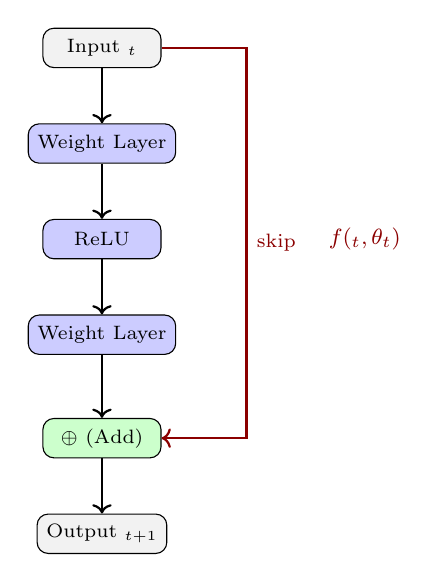
\begin{tikzpicture}[scale=0.9, node distance=0.8cm and 1.2cm, every node/.style={font=\scriptsize}]
  \node[draw, fill=gray!10, rounded corners, minimum width=1.5cm, minimum height=0.5cm] (in) {Input $\hbf_t$};
  \node[draw, fill=blue!20, rounded corners, minimum width=1.5cm, minimum height=0.5cm, below=0.7cm of in] (w1) {Weight Layer};
  \node[draw, fill=blue!20, rounded corners, minimum width=1.5cm, minimum height=0.5cm, below=0.7cm of w1] (relu) {ReLU};
  \node[draw, fill=blue!20, rounded corners, minimum width=1.5cm, minimum height=0.5cm, below=0.7cm of relu] (w2) {Weight Layer};
  \node[draw, fill=green!20, rounded corners, minimum width=1.5cm, minimum height=0.5cm, below=0.8cm of w2] (add) {$\oplus$ (Add)};
  \node[draw, fill=gray!10, rounded corners, minimum width=1.5cm, minimum height=0.5cm, below=0.7cm of add] (out) {Output $\xbf_{t+1}$};
  \draw[->, thick] (in) -- (w1);
  \draw[->, thick] (w1) -- (relu);
  \draw[->, thick] (relu) -- (w2);
  \draw[->, thick] (w2) -- (add);
  \draw[->, thick] (add) -- (out);
  % Skip connection
  \draw[->, thick, DarkRed] (in.east) -- ++(1.2,0) |- (add.east) node[pos=0.25, right, DarkRed] {skip};
  \node[right=2.0cm of relu, text=DarkRed, font=\footnotesize] {$f(\xbf_t, \theta_t)$};
\end{tikzpicture}
\end{columns}
\end{frame}
 
%--------------------------------------------------------------
\begin{frame}{From Discrete to Continuous Depth}

\scriptsize

\begin{tblockFrost}{}
As number of layers $T \to \infty$ and step size $\Delta t \to 0$, the residual update
$$
  \xbf_{t+1} = \xbf_t + \Delta t\, f(\xbf_t,\, t,\, \theta)
$$
converges to the \textbf{continuous ODE}:
$$
  \boxed{\frac{d\xbf(t)}{dt} = f\!\left(\xbf(t),\, t,\, \theta\right)}
$$
\end{tblockFrost}
\begin{columns}
\column{0.48\textwidth}
\begin{block}{Discrete: ResNet}
$$
  \xbf_T = \xbf_0 + \sum_{t=0}^{T-1} f(\xbf_t, \theta_t)
$$
\end{block}
\column{0.48\textwidth}
\begin{block}{Continuous: Neural ODE}
$$
  \xbf(T) = \xbf(0) + \int_0^T f\!\left(\xbf(t), t, \theta\right) dt
$$
\end{block}
\end{columns}
\vspace{6pt}
\begin{alertblock}{}
The parameters $\theta$ are \textbf{shared across all depths}, unlike ResNets with per-layer weights. This gives \textbf{constant parameter count} regardless of integration depth.
\end{alertblock}
\end{frame}

 
%==============================================================
\section{Mathematical Foundations}
%==============================================================
 
\begin{frame}{Ordinary Differential Equations (ODEs)}

\scriptsize

\begin{columns}
\column{0.52\textwidth}
\begin{tblockFrost}{Initial Value Problem (IVP)}
Given dynamics $f$ and initial condition $\xbf(t_0) = \xbf_0$, find $\xbf(t)$:
$$
  \frac{d\xbf}{dt} = f(\xbf(t), t), \quad \xbf(t_0) = \xbf_0
$$
\textbf{Solution} (via Picard–Lindelöf):
$$
  \xbf(t) = \xbf_0 + \int_{t_0}^{t} f(\xbf(s), s)\, ds
$$
\end{tblockFrost}
\begin{block}{Existence \& Uniqueness}
If $f$ is \textbf{Lipschitz continuous} in $\hbf$, a unique solution exists on $[t_0, T]$.
\end{block}
\column{0.44\textwidth}
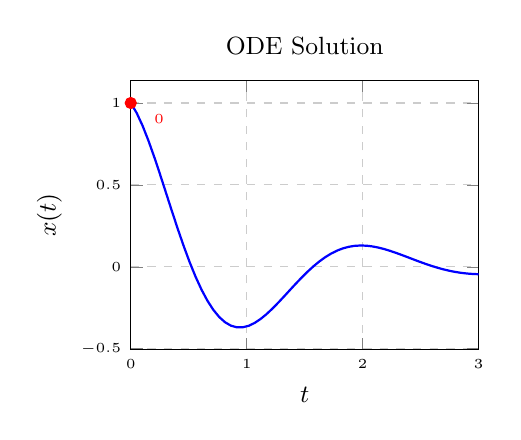
\begin{tikzpicture}
\begin{axis}[
  width=6cm, height=5cm,
  xlabel={$t$}, ylabel={$x(t)$},
  title={\small ODE Solution},
  grid=major, grid style={dashed, gray!40},
  title style={font=\small},
  tick label style={font=\tiny},
  label style={font=\small},
  xmin=0, xmax=3,
]
\addplot[thick, blue, domain=0:3, samples=60] {exp(-x)*cos(deg(3*x))};
\addplot[only marks, mark=*, mark size=2pt, red] coordinates {(0,1)};
\node[font=\tiny, red] at (axis cs:0.25, 0.9) {$\xbf_0$};
\end{axis}
\end{tikzpicture}
\end{columns}
\end{frame}

%--------------------------------------------------------------
\begin{frame}{Numerical ODE Solvers}
\scriptsize
\begin{columns}
\column{0.50\textwidth}
\begin{tblockWing}{Euler Method (1st Order)}
\vspace{-20pt}
\begin{align*}
  \xbf_{t+h} \approx \xbf_t + h\, f(\xbf_t, t)
\end{align*}

Simple but low accuracy; $\mathcal{O}(h)$ error per step.
\end{tblockWing}
\vspace{2pt}
\begin{tblockWing}{Runge-Kutta 4 (RK4)}
\vspace{-20pt}
\begin{align*}
  k_1 &= f(\xbf_t,\, t)\\
  k_2 &= f\!\left(\xbf_t + \tfrac{h}{2}k_1,\, t+\tfrac{h}{2}\right)\\
  k_3 &= f\!\left(\xbf_t + \tfrac{h}{2}k_2,\, t+\tfrac{h}{2}\right)\\
  k_4 &= f(\xbf_t + h\, k_3,\, t+h)\\
  \xbf_{t+h} &= \xbf_t + \tfrac{h}{6}(k_1 + 2k_2 + 2k_3 + k_4)
\end{align*}
$\mathcal{O}(h^4)$ error per step.
\end{tblockWing}
\column{0.46\textwidth}
\begin{tblockWing}{Adaptive Solvers (Dopri5)}
\begin{itemize}
  \item Embed two RK schemes of different orders
  \item Estimate local truncation error
  \item \textbf{Increase} step size when error is small
  \item \textbf{Decrease} step size when error is large
  \item Control solution to a user-specified tolerance: \texttt{rtol}, \texttt{atol}
\end{itemize}
\end{tblockWing}
\vspace{4pt}
\begin{alertblock}{}
Neural ODE dynamics can vary rapidly in some regions; adaptive solvers allocate computation where needed, yielding efficiency and accuracy.
\end{alertblock}
\end{columns}
\end{frame}

%==============================================================
\section{Neural ODEs}
%==============================================================
 
\begin{frame}{Introducing Neural ODEs}
\scriptsize
\begin{tblockFrost}{Definition}
A \textbf{Neural ODE} parametrizes the derivative of a hidden state with a neural network $f_\theta$:
$$
  \frac{d\xbf(t)}{dt} = f_\theta\!\left(\xbf(t),\, t\right), \qquad \xbf(t_0) = \xbf_0
$$
The output at time $t_1$ is computed by \textbf{numerically integrating} the ODE:
$$
  \xbf(t_1) = \xbf(t_0) + \int_{t_0}^{t_1} f_\theta\!\left(\xbf(t), t\right) dt
  \;=\; \texttt{ODESolve}(f_\theta,\, \xbf_0,\, t_0,\, t_1)
$$
\end{tblockFrost}
\vspace{4pt}
\begin{columns}
\column{0.48\textwidth}
\begin{block}{Forward Pass}
\begin{enumerate}
  \item Set initial state $\xbf(t_0)$ (e.g., encoder output)
  \item Call ODE solver with $f_\theta$
  \item Obtain $\xbf(t_1)$ as the model output
  \item Apply output layer / loss
\end{enumerate}
\end{block}
\column{0.48\textwidth}
\begin{block}{Backward Pass}
\begin{enumerate}
  \item Do \textbf{NOT} backprop through solver steps
  \item Solve a \textbf{reverse-time ODE} (adjoint)
  \item Compute gradients $\nabla_\theta \mathcal{L}$ efficiently
  \item Memory cost: $\mathcal{O}(1)$ in depth
\end{enumerate}
\end{block}
\end{columns}
\end{frame}

%--------------------------------------------------------------
\begin{frame}{Neural ODE: Architecture View}
\begin{center}
\resizebox{0.8\linewidth}{!}{
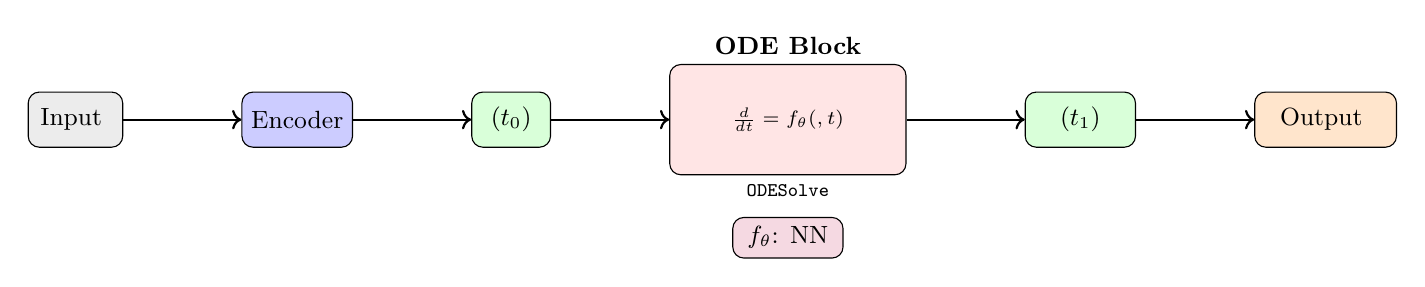
\begin{tikzpicture}[scale=0.6, node distance=0.6cm and 0.4cm, every node/.style={font=\small}]
  % Input
  \node[draw, fill=gray!15, rounded corners, minimum width=1.2cm, minimum height=0.7cm] (input) {Input $\xbf$};
  % Encoder
  \node[draw, fill=blue!20, rounded corners, minimum width=1.2cm, minimum height=0.7cm, right=1.5cm of input] (enc) {Encoder};
  % h0
  \node[draw, fill=green!15, rounded corners, minimum width=1.0cm, minimum height=0.7cm, right=1.5cm of enc] (h0) {$\xbf(t_0)$};
  % ODE block
  \node[draw, fill=red!10, rounded corners, minimum width=3cm, minimum height=1.4cm, right=1.5cm of h0] (ode) {};
  \node[above] at (ode.north) {\textbf{ODE Block}};
  \node[font=\scriptsize] at (ode.center) {$\frac{d\xbf}{dt}=f_\theta(\xbf,t)$};
  \node[font=\scriptsize, below=0pt] at (ode.south) {\texttt{ODESolve}};
  % h1
  \node[draw, fill=green!15, rounded corners, minimum width=1.4cm, minimum height=0.7cm, right=1.5cm of ode] (h1) {$\xbf(t_1)$};
  % Output
  \node[draw, fill=orange!20, rounded corners, minimum width=1.8cm, minimum height=0.7cm, right=1.5cm of h1] (out) {Output $\ybf$};
  % Arrows
  \draw[->, thick] (input) -- (enc);
  \draw[->, thick] (enc) -- (h0);
  \draw[->, thick] (h0) -- (ode);
  \draw[->, thick] (ode) -- (h1);
  \draw[->, thick] (h1) -- (out);
  % f_theta label inside ODE block
  \node[draw, fill=purple!15, rounded corners, minimum width=1.4cm, minimum height=0.5cm] at ([yshift=-2.5cm]ode.center) {$f_\theta$: NN};
\end{tikzpicture}
}
\end{center}
\vspace{4pt}
\begin{columns}
\column{0.48\textwidth}
\begin{tblockFrost}{Continuous Depth}
The ``depth'' of the network is the integration interval $[t_0, t_1]$. More complex inputs naturally require more solver steps (adaptive depth).
\end{tblockFrost}
\column{0.48\textwidth}
\begin{tblockFrost}{Parameter Efficiency}
$f_\theta$ is \textbf{shared} across all integration steps. Total parameters determined by the architecture of $f_\theta$, \emph{not} by integration depth.
\end{tblockFrost}
\end{columns}
\end{frame}


\begin{frame}{}

\begin{center}
\includegraphics[width=0.5\linewidth]{figures/odenet.png}
\end{center}

\end{frame}

%--------------------------------------------------------------
\begin{frame}{Neural ODE for Classification}
\scriptsize

\begin{columns}
\column{0.52\textwidth}
\begin{tblockWing}{}
\begin{enumerate}
  \item \textbf{Downsampling conv layers}: extract features from input image $\xbf$
  \item \textbf{ODE block}: continuous feature evolution
$$
    \frac{d\xbf}{dt} = f_\theta(\xbf(t), t)
$$
  \item \textbf{Fully connected layer}: map $\xbf(t_1) \to$ class logits
\end{enumerate}
\end{tblockWing}
\vspace{4pt}

\column{0.44\textwidth}
\begin{tblockWing}{ODE block is invertible.}
Given $\xbf(t_1)$, integrate the ODE \textbf{backwards} in time from $t_1$ to $t_0$:
$$
  \xbf(t_0) = \xbf(t_1) + \int_{t_1}^{t_0} f_\theta(\xbf(t), t)\, dt
$$
This gives exact \textbf{free invertibility}, an interesting property for normalizing flows!
\end{tblockWing}
\end{columns}

\end{frame}

%==============================================================
\section{Adjoint Sensitivity Method}
%==============================================================

\begin{frame}{Difficult of Bakcpropagaion in Neural ODE}

\begin{center}



Backpropagation (or reverse mode differentiation as you can call it) is difficult for continuous-depth networks.


We treat ODE as a blackbox and compute gradients using \textbf{adjoint sensitivity} method that dates back to 1962. 

Adjoint senstivity method computes gradients by solving  second, augmented ODE backwards in time, and is applicable to all ODE solvers.



\end{center}

\end{frame}
 
\begin{frame}{The Adjoint Sensitivity Method: Overview}
\scriptsize

\begin{tblockFrost}{The Problem}
To get trained model with parameters $\theta$ we need $\frac{d\mathcal{L}}{d\theta}$. Naively backpropping through the ODE solver requires storing all intermediate states $\Rightarrow$ $\mathcal{O}(N_{\text{steps}})$ memory.
\end{tblockFrost}
\vspace{4pt}
\begin{block}{Adjoint State}
Define the \textbf{adjoint} $\abf(t) = \frac{\partial \mathcal{L}}{\partial \xbf(t)}$.
\begin{itemize}
  \item $\abf(t_1) = \frac{\partial \mathcal{L}}{\partial \xbf(t_1)}$ (from loss at output)
  \item $\abf(t)$ evolves \textbf{backwards} via its own ODE:
\end{itemize}
$$
  \frac{d\abf(t)}{dt} = -\abf(t)^\T \frac{\partial f_\theta(\xbf(t), t, \theta)}{\partial \xbf(t)}
$$
\end{block}
\vspace{4pt}
\begin{alertblock}{}
The adjoint ODE is solved \textbf{backwards in time}, recomputing $\xbf(t)$ on the fly. No need to store forward trajectory. Memory cost: $\mathcal{O}(1)$ (constant w.r.t.\ solver steps)!
\end{alertblock}
\end{frame}



\begin{frame}{Adjoint Method: Gradient Computation}
\scriptsize


\begin{itemize}
\item We can compute $\pdv{\Lcal}{\xbf(t_0)}$ by another call to ODE solver.

\item This solver must run backwards starting from the initial value of $\pdv{\Lcal}{\xbf(t_1)}$.

\item This may require knowing $\xbf(t)$  along its entire trajectory.

\item But we can simply recompute $\xbf(t)$ backwards in time together with the adjoint starting from its final value $\xbf(t_1)$.
\end{itemize}

Computing the gradient wrt $\theta$ requires evaluating a third integral which depends on both $\zbf(t)$ and $\abf(t)$:

\begin{align*}
\frac{d\Lcal}{d\theta} = -\int_{t_1}^{t_0} \abf^\top \frac{\partial f_\theta(\xbf(t), t, \theta)}{\partial \xbf(t)} dt
\end{align*}

\end{frame}


\begin{frame}{}

\begin{center}
\includegraphics[width=0.4\linewidth]{figures/adjoint_sensitivity.png}

\url{https://arxiv.org/pdf/1806.07366}

\end{center}

\end{frame}
%--------------------------------------------------------------
\begin{frame}{Adjoint Method: Gradient Computation}
\scriptsize


\begin{columns}
\column{0.48\textwidth}

\begin{tblockFrost}{Augmented ODE (Backward in Time)}
Solve the following augmented system from $t_1$ to $t_0$:
$$
  \frac{d}{dt}\begin{bmatrix}\xbf(t)\\ \abf(t)\\ \frac{d\mathcal{L}}{d\theta}\end{bmatrix}
  = \begin{bmatrix}
      f_\theta(\xbf, t)\\
      -\abf^\T \frac{\partial f_\theta}{\partial \xbf}\\
      -\abf^\T \frac{\partial f_\theta}{\partial \theta}
    \end{bmatrix}
$$
with initial conditions at $t_1$:
$$
  \xbf(t_1),\quad \abf(t_1) = \frac{\partial \mathcal{L}}{\partial \xbf(t_1)}, \quad \frac{d\mathcal{L}}{d\theta}\bigg|_{t_1} = \mathbf{0}
$$
\end{tblockFrost}

\begin{block}{After integrating to $t_0$:}
\begin{itemize}
  \item $\abf(t_0) = \frac{\partial \mathcal{L}}{\partial \xbf(t_0)}$ \quad (gradient w.r.t.\ initial state)
  \item $\frac{d\mathcal{L}}{d\theta}$ accumulated across all time \quad (gradient w.r.t.\ parameters)
\end{itemize}
\end{block}
\column{0.48\textwidth}
\begin{tblockWing}{Computation Summary}
\begin{tabular}{lc}
\toprule
Quantity & Cost\\
\midrule
Forward solve & 1 ODE call\\
Backward solve & 1 ODE call\\
Memory & $\mathcal{O}(1)$\\
Jacobian-vecs & via autograd\\
\bottomrule
\end{tabular}
\end{tblockWing}
\end{columns}
\end{frame}

\begin{frame}{Adjoint Method: Algorithm}
\scriptsize

\begin{algorithm}[H]
\caption{Neural ODE Training with Adjoint Sensitivity}
\SetAlgoLined
\KwIn{Parameters $\theta$, initial state $\xbf_0$, loss $\mathcal{L}$, times $t_0 < t_1$}
\KwOut{Gradients $\frac{d\mathcal{L}}{d\theta}$, $\frac{d\mathcal{L}}{d\xbf_0}$}
\BlankLine
\textbf{Forward pass:}\\
$\xbf(t_1) \leftarrow \texttt{ODESolve}(f_\theta, \xbf_0, t_0, t_1)$\;
Compute $\mathcal{L}(\xbf(t_1))$\;
\BlankLine
\textbf{Backward pass (Adjoint):}\\
Initialize $\abf(t_1) = \frac{\partial \mathcal{L}}{\partial \xbf(t_1)}$,\; $\gbf_\theta = \mathbf{0}$\;
Solve augmented ODE from $t_1$ to $t_0$:
$[\hbf(t_0),\, \abf(t_0),\, \gbf_\theta] \leftarrow \texttt{ODESolve}(\text{aug}, [\xbf_1, \abf_1, \mathbf{0}], t_1, t_0)$\;
\Return $\frac{d\mathcal{L}}{d\xbf_0} = \abf(t_0)$,\;\; $\frac{d\mathcal{L}}{d\theta} = \gbf_\theta$\;
\end{algorithm}
\vspace{4pt}
\begin{alertblock}{}
The backward augmented ODE is solved with the \emph{same} ODE solver as the forward pass, the solver is a black box, gradients flow through the \textbf{adjoint ODE}, not through solver steps.
\end{alertblock}
\end{frame}

%==============================================================
\section{Continuous Normalizing Flows}
%==============================================================
 
\begin{frame}{Normalizing Flows: Background}

\scriptsize

\begin{columns}
\column{0.50\textwidth}
\begin{tblockFrost}{Change of Variables}
A normalizing flow maps a simple base distribution $p_z(\zbf)$ (e.g., Gaussian) to a complex target $p_x(\xbf)$ via an invertible map $g: \zbf \mapsto \xbf$:

$$
\xbf = f(\zbf) \Rightarrow  \log p_x(\xbf) = \log p_z(\zbf) - \log \left|\det \frac{\partial g}{\partial \zbf}\right|
$$
\end{tblockFrost}
\vspace{4pt}
\begin{tblockWing}{Discrete NF Challenges}
\begin{itemize}
  \item Must design \textbf{special invertible architectures}
  \item Jacobian determinant computation: $\mathcal{O}(d^3)$ in general
  \item Coupling layers restrict architecture freedom
\end{itemize}
\end{tblockWing}
\column{0.46\textwidth}
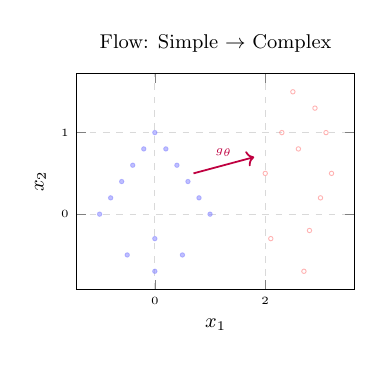
\begin{tikzpicture}[scale=0.8]
  \begin{axis}[
    width=6cm, height=5cm,
    xlabel={$x_1$}, ylabel={$x_2$},
    title={\small Flow: Simple $\to$ Complex},
    grid=major, grid style={dashed, gray!30},
    tick label style={font=\tiny},
    label style={font=\small},
    title style={font=\small},
  ]
  \addplot[only marks, mark=*, mark size=1pt, blue!50, opacity=0.5]
    coordinates {
      (-1,0)(-0.8,0.2)(-0.6,0.4)(-0.4,0.6)(-0.2,0.8)(0,1)(0.2,0.8)(0.4,0.6)(0.6,0.4)(0.8,0.2)(1,0)
      (-0.5,-0.5)(0,-0.7)(0.5,-0.5)(0,-0.3)
    };
  \addplot[only marks, mark=o, mark size=1pt, red!60, opacity=0.5]
    coordinates {
      (2,0.5)(2.3,1.0)(2.6,0.8)(2.9,1.3)(3.2,0.5)(2.1,-0.3)(2.8,-0.2)(3.0,0.2)
      (2.5,1.5)(2.7,-0.7)(3.1,1.0)
    };
  \draw[->, thick, purple] (axis cs:0.7, 0.5) -- (axis cs:1.8, 0.7) node[midway, above, font=\tiny] {$g_\theta$};
  \end{axis}
\end{tikzpicture}
\end{columns}
\end{frame}
 
 
\begin{frame}{Continuous Normalizing Flows (CNF)}

\scriptsize

\begin{tblockFrost}{Instantaneous Change of Variables}
For a continuous transformation $\zbf(t)$ governed by an ODE, the log-density evolves as:
$$
  \frac{\partial \log p(\zbf(t))}{\partial t} = -\operatorname{tr}\!\left(\frac{\partial f_\theta}{\partial \zbf(t)}\right)
$$
This is the \textbf{instantaneous change of variables} formula (Liouville's theorem).
\end{tblockFrost}
\vspace{4pt}
\begin{columns}
\column{0.48\textwidth}
\begin{block}{CNF Log-Likelihood}
$$
  \log p(\xbf) = \log p(\zbf(t_0)) - \int_{t_0}^{t_1} \operatorname{tr}\!\left(\frac{\partial f_\theta}{\partial \zbf}\right) dt
$$
\begin{itemize}
  \item $p(\zbf(t_0))$: base density (Gaussian)
  \item Trace computable in $\mathcal{O}(d)$ via Hutchinson's estimator
\end{itemize}
\end{block}
\column{0.48\textwidth}
\begin{golden}{Advantages over Discrete NF}
\begin{itemize}
  \item \textbf{Free-form} $f_\theta$, no special invertibility constraints
  \item Only \textbf{trace} (not full Jacobian) needed
  \item Can model highly complex distributions
  \item Generation: integrate ODE forward; inference: backward
\end{itemize}
\end{golden}
\end{columns}
\end{frame}
 
 
 \begin{frame}{Hutchinson's Trace Estimator}
 \scriptsize
 
\begin{block}{Problem}
Computing $\operatorname{tr}(J_f)$ where $J_f = \frac{\partial f_\theta}{\partial \zbf} \in \Rbb^{d \times d}$ costs $\mathcal{O}(d^2)$, expensive for large $d$!
\end{block}
\vspace{6pt}
\begin{tblockFrost}{Hutchinson Estimator}
For any random vector $\varepsilon \in \Rbb^d$ with $\Ebb[\varepsilon] = 0$, $\Ebb[\varepsilon \varepsilon^\T] = I$:
$$
  \operatorname{tr}(J_f) = \Ebb_{\varepsilon}\!\left[\varepsilon^\T J_f\, \varepsilon\right]
$$
\begin{itemize}
  \item $\varepsilon^\T J_f$ is a \textbf{vector-Jacobian product}: computable via one backward pass through $f_\theta$, costing $\mathcal{O}(d)$
  \item Use Rademacher noise: $\varepsilon_i \in \{-1, +1\}$ with equal probability
  \item Average over $K$ samples for low-variance estimate
\end{itemize}
\end{tblockFrost}
\begin{alertblock}{}
Training CNFs requires only $\mathcal{O}(d)$ operations per step, making high-dimensional density estimation tractable.
\end{alertblock}
\end{frame}

%==============================================================
\section{Latent Neural ODEs}
%==============================================================
 
\begin{frame}{Latent Neural ODEs for Time Series}
\scriptsize

\begin{tblockFrost}{Motivation: Irregular Time Series}
Standard RNNs process observations at fixed, regular intervals. Real-world data is:
\begin{itemize}
  \item \textbf{Irregularly sampled}: medical records, sensor readings
  \item \textbf{Partially observed}: missing measurements
  \item \textbf{Multi-rate}: different sensors at different frequencies
\end{itemize}
\end{tblockFrost}
\vspace{4pt}
\begin{columns}
\column{0.50\textwidth}
\begin{tblockWing}{Latent ODE Model}
\begin{enumerate}
  \item \textbf{Encoder} (ODE-RNN): infer initial latent state $\zbf(t_0)$ from observations
  \item \textbf{Latent dynamics}: $\frac{d\zbf}{dt} = f_\theta(\zbf(t))$ (no explicit $t$-dependence)
  \item \textbf{Decoder}: map latent $\zbf(t_k) \to \hat{\xbf}(t_k)$ at any time $t_k$
\end{enumerate}
\end{tblockWing}
\column{0.46\textwidth}
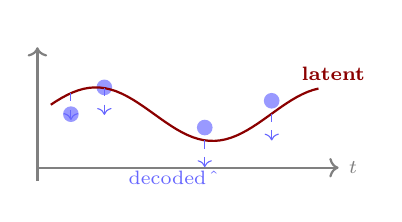
\begin{tikzpicture}[scale=0.85, every node/.style={font=\scriptsize}]
  % observations
  \foreach \t/\x in {0.5/0.8, 1.0/1.2, 2.5/0.6, 3.5/1.0}{
    \node[circle, fill=blue!40, inner sep=2pt] at (\t, \x) {};
  }
  \draw[->, thick, gray] (0,0) -- (4.5,0) node[right] {$t$};
  \draw[->, thick, gray] (0,-0.2) -- (0,1.8) node[above] {$\xbf$};
  % continuous latent
  \draw[thick, DarkRed, domain=0.2:4.2, samples=50]
    plot (\x, {0.8 + 0.4*sin(deg(1.8*\x))});
  \node[DarkRed, right] at (3.8, 1.4) {\textbf{latent}};
  % decoder arrows
  \foreach \t in {0.5, 1.0, 2.5, 3.5}{
    \draw[->, dashed, blue!60] (\t, {0.8+0.4*sin(deg(1.8*\t))}) -- (\t, {0.8+0.4*sin(deg(1.8*\t))-0.4});
  }
  \node[blue!60] at (2.0, -0.15) {decoded $\hat{\xbf}$};
\end{tikzpicture}
\end{columns}
\end{frame}


\begin{frame}{ODE-RNN Encoder}
\scriptsize

\begin{columns}
\column{0.52\textwidth}
\begin{tblockFrost}{ODE-RNN}
Combine an RNN (for observation updates) with an ODE (for dynamics between observations):
\begin{itemize}
  \item At observation time $t_k$: \textbf{RNN update}
$$
    \hbf(t_k^+) = \text{RNNCell}\!\left(\hbf(t_k^-),\, \xbf(t_k)\right)
$$
  \item Between observations: \textbf{ODE evolution}
$$
    \hbf(t_{k+1}^-) = \texttt{ODESolve}(f_\theta, \hbf(t_k^+), t_k, t_{k+1})
$$
\end{itemize}
\end{tblockFrost}
\begin{alertblock}{}
Handles \textbf{arbitrarily irregular} time gaps between observations naturally.
\end{alertblock}
\column{0.44\textwidth}
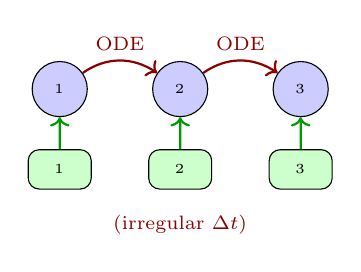
\begin{tikzpicture}[scale=0.85, every node/.style={font=\scriptsize}, node distance=0.6cm]
  \foreach \i/\t in {1/$t_1$, 2/$t_2$, 3/$t_3$}{
    \node[draw, fill=blue!20, circle, minimum size=0.7cm] (h\i) at (\i*1.8, 0) {$\hbf_{\i}$};
    \node[draw, fill=green!20, rectangle, rounded corners, minimum width=0.8cm, minimum height=0.5cm] (x\i) at (\i*1.8, -1.2) {$\xbf_{\i}$};
    \draw[->, thick, green!60!black] (x\i) -- (h\i);
  }
  % ODE arcs between RNN nodes
  \draw[->, thick, DarkRed, bend left=35] (h1) to node[above, midway] {\scriptsize ODE} (h2);
  \draw[->, thick, DarkRed, bend left=35] (h2) to node[above, midway] {\scriptsize ODE} (h3);
  \node[below=0.2cm of x2, DarkRed] {(irregular $\Delta t$)};
\end{tikzpicture}
\end{columns}
\end{frame}

\begin{frame}{Latent ODE: Generative Model}
\scriptsize

\begin{tblockFrost}{Variational Formulation}
Model observations as:
$$
  \zbf(t_0) \sim p(\zbf_0), \quad
  \zbf(t) = \zbf(t_0) + \int_{t_0}^{t} f_\theta(\zbf(s))\, ds, \quad
  \xbf(t_k) \sim p(\xbf \mid \zbf(t_k))
$$
Train with \textbf{ELBO} (Evidence Lower Bound):
$$
  \mathcal{L} = \Ebb_{q(\zbf_0 | \{\xbf(t_k)\})}\!\left[\sum_k \log p(\xbf(t_k) \mid \zbf(t_k))\right] - \text{KL}\!\left[q(\zbf_0 \mid \cdot) \;\|\; p(\zbf_0)\right]
$$
\end{tblockFrost}
\vspace{4pt}
\begin{columns}
\column{0.48\textwidth}
\begin{block}{Capabilities}
\begin{itemize}
  \item Interpolate at \textbf{any time} (not just observed)
  \item Extrapolate into future
  \item Handle \textbf{missing data} gracefully
  \item Uncertainty quantification
\end{itemize}
\end{block}
\column{0.48\textwidth}
\begin{block}{Applications}
\begin{itemize}
  \item Clinical time series (ICU data)
  \item Physical system identification
  \item Financial time series
  \item Motion capture / trajectory modeling
\end{itemize}
\end{block}
\end{columns}
\end{frame}

%==============================================================
\section{Implementation}
%==============================================================
 
\begin{frame}[fragile]{Implementation with \texttt{torchdiffeq}}
\scriptsize

\begin{columns}

\column{0.4\linewidth}



\begin{tblockFrost}{\texttt{torchdiffeq} Library (Chen et al.)}
\begin{itemize}
  \item PyTorch-based library for differentiable ODE solving
  \item Supports: \texttt{euler}, \texttt{rk4}, \texttt{dopri5} (Dormand–Prince), \texttt{adams}
  \item Automatic adjoint-based gradients
\end{itemize}
\end{tblockFrost}

\column{0.5\linewidth}



\begin{minted}[
    linenos,
    frame=lines,
    framesep=2mm,
    bgcolor=pink!10,
    fontsize=\tiny,
    breaklines
]{Python}
from torchdiffeq import odeint, odeint_adjoint
import torch, torch.nn as nn
 
class ODEFunc(nn.Module):
    """Parametrize dh/dt = f_theta(h, t)"""
    def __init__(self, hidden_dim):
        super().__init__()
        self.net = nn.Sequential(
            nn.Linear(hidden_dim, hidden_dim),
            nn.Tanh(),
            nn.Linear(hidden_dim, hidden_dim),
        )
    def forward(self, t, h):   # Note: signature must be (t, h)
        return self.net(h)
 
func = ODEFunc(hidden_dim=64)
h0   = torch.randn(16, 64)          # batch_size x hidden_dim
t    = torch.tensor([0.0, 1.0])     # integration interval
# odeint_adjoint uses O(1) memory backprop
h1   = odeint_adjoint(func, h0, t, method='dopri5')[-1]
\end{minted}

\end{columns}

\end{frame}
 
%--------------------------------------------------------------
\begin{frame}[fragile]{Complete Neural ODE Classifier}


\begin{minted}[
    linenos,
    frame=lines,
    framesep=2mm,
    bgcolor=pink!10,
    fontsize=\tiny,
    breaklines
]{Python}
class NeuralODEClassifier(nn.Module):
    def __init__(self, in_dim=784, hidden=64, n_classes=10):
        super().__init__()
        self.encoder  = nn.Linear(in_dim, hidden)
        self.ode_func = ODEFunc(hidden)
        self.decoder  = nn.Linear(hidden, n_classes)
        self.t        = torch.tensor([0.0, 1.0])
    def forward(self, x):
        h0 = self.encoder(x)                          # (B, hidden)
        # Solve ODE: O(1) memory, adaptive steps
        hT = odeint_adjoint(self.ode_func, h0,
                             self.t, method='dopri5')[-1]
        return self.decoder(hT)                       # logits
# Training loop (standard)
model     = NeuralODEClassifier()
optimizer = torch.optim.Adam(model.parameters(), lr=1e-3)
criterion = nn.CrossEntropyLoss()
for x_batch, y_batch in dataloader:
    logits = model(x_batch.view(x_batch.size(0), -1))
    loss   = criterion(logits, y_batch)
    optimizer.zero_grad()
    loss.backward()      # adjoint handles backprop
    optimizer.step()
\end{minted}

\end{frame}
 
%--------------------------------------------------------------
\begin{frame}[fragile]{ODE Solver Options in \texttt{torchdiffeq}}
\scriptsize

\begin{columns}
\column{0.50\textwidth}
\begin{tblockFrost}{Available Solvers}
\begin{tabular}{ll}
\toprule
\textbf{Method} & \textbf{Order / Type}\\
\midrule
\texttt{euler}    & 1st, fixed-step\\
\texttt{midpoint} & 2nd, fixed-step\\
\texttt{rk4}      & 4th, fixed-step\\
\texttt{dopri5}   & 4/5th, adaptive\\
\texttt{dopri8}   & 8th, adaptive\\
\texttt{adams}    & multi-step, adaptive\\
\texttt{bosh3}    & 2/3rd, adaptive\\
\bottomrule
\end{tabular}
\end{tblockFrost}

\begin{alertblock}{}
Use \texttt{dopri5} for training (accuracy), \texttt{rk4} with fixed step for fast inference.
\end{alertblock}

\column{0.46\textwidth}
\begin{MintedFrame}
\begin{minted}{python}
# Tight tolerances for high accuracy
h = odeint_adjoint(
    func, h0, t,
    method='dopri5',
    rtol=1e-5,
    atol=1e-6
)
 
# Faster inference: fixed-step
h = odeint(
    func, h0, t,
    method='rk4',
    options={'step_size': 0.1}
)
\end{minted}
\end{MintedFrame}

\end{columns}
\end{frame}
 
%==============================================================
\section{Advantages and Limitations}
%==============================================================
 
\begin{frame}{Advantages of Neural ODEs}
\scriptsize

\begin{columns}
\column{0.50\textwidth}
\begin{tblockWing}{Core Strengths}
\begin{enumerate}
  \item[\faFlash] \textbf{Memory Efficiency}\\
    Adjoint backprop: $\mathcal{O}(1)$ memory vs.\ $\mathcal{O}(L)$ for ResNet
  \vspace{2pt}
  \item[\faFlash] \textbf{Adaptive Computation}\\
    ODE solver uses more steps for complex regions; fewer steps where dynamics are simple
  \vspace{2pt}
  \item[\faFlash] \textbf{Continuous Dynamics}\\
    Outputs defined at \emph{any} time $t \in [t_0, t_1]$, not just integer layers
  \vspace{2pt}
  \item[\faFlash] \textbf{Invertibility}\\
    Free inversion via backward ODE integration — crucial for generative models
\end{enumerate}
\end{tblockWing}
\column{0.46\textwidth}
\begin{tblockWing}{Application-Specific Gains}
\begin{enumerate}
  \item[\faFlash] \textbf{Irregular Time Series}\\
    Handles variable time gaps naturally
  \vspace{2pt}
  \item[\faFlash] \textbf{Continuous Normalizing Flows}\\
    Exact log-likelihood with free-form architecture
  \vspace{2pt}
  \item[\faFlash] \textbf{Parameter Efficiency}\\
    Weights shared across all "depths" (integration steps)
  \vspace{2pt}
  \item[\faFlash] \textbf{Physical Inductive Bias}\\
    Natural fit for systems governed by differential equations (mechanics, chemistry, biology)
\end{enumerate}
\end{tblockWing}
\end{columns}
\end{frame}
 
%--------------------------------------------------------------
\begin{frame}{Limitations and Challenges}
\scriptsize
\begin{columns}
\column{0.48\textwidth}
\begin{tblockWing}{Computational Challenges}
\begin{itemize}
  \item \textbf{Slow training}: ODE solving is iterative; each gradient step requires forward + backward ODE integration
  \item \textbf{Stiff ODEs}: dynamics with very different timescales require tiny step sizes
  \item \textbf{Adjoint inaccuracy}: numerical errors in backward ODE accumulate; tight tolerances needed
  \item \textbf{Depth-accuracy tradeoff}: coarser tolerance $\Rightarrow$ fewer steps but less accurate
\end{itemize}
\end{tblockWing}
\column{0.48\textwidth}
\begin{tblockWing}{Modeling Limitations}
\begin{itemize}
  \item \textbf{No crossing trajectories}: homeomorphism constraint — the ODE flow is a diffeomorphism; cannot fold or cross in latent space
  \item \textbf{Topology}: cannot change topology of data manifold (e.g., cannot map one cluster to two disjoint clusters without augmentation)
  \item \textbf{Expressiveness}: augment state space to overcome (Augmented Neural ODEs)
  \item \textbf{Hyperparameter sensitivity}: solver tolerance, integration range need tuning
\end{itemize}
\end{tblockWing}
\end{columns}
\end{frame}
 
%--------------------------------------------------------------
\begin{frame}{Augmented Neural ODEs}

\scriptsize

\begin{tblockFrost}{Motivation: Overcoming Topology Limitations}
Recall: an ODE flow $\phi: \Rbb^d \to \Rbb^d$ is a \textbf{homeomorphism} — cannot change topology. For example, points on opposite sides of a boundary cannot swap during integration (no crossing).
\end{tblockFrost}
\vspace{4pt}
\begin{columns}
\column{0.52\textwidth}
\begin{block}{Augmented Neural ODE (ANODE)}
Augment the state with $p$ additional dimensions initialized to zero:
$$
  \tilde{\xbf}(t_0) = \begin{bmatrix} \xbf(t_0) \\ \mathbf{0}_p \end{bmatrix} \in \Rbb^{d+p}
$$
Solve the ODE in the augmented space $\Rbb^{d+p}$, then read off the first $d$ dimensions.
\begin{itemize}
  \item Extra dimensions provide ``lifting'' room to route around topological barriers
  \item Small $p$ (e.g., $p = 1$) often sufficient in practice
\end{itemize}
\end{block}
\column{0.44\textwidth}
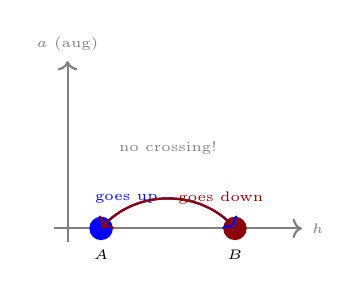
\begin{tikzpicture}[scale=0.85]
  % 1D -> 2D augmentation illustration
  \draw[->, thick, gray] (-0.2,0) -- (3.5,0) node[right, font=\tiny] {$h$};
  \draw[->, thick, gray] (0,-0.2) -- (0,2.5) node[above, font=\tiny] {$a$ (aug)};
  % Two points that need to swap in 1D
  \node[circle, fill=blue, inner sep=3pt, label=below:{\tiny $A$}] at (0.5,0) {};
  \node[circle, fill=DarkRed, inner sep=3pt, label=below:{\tiny $B$}] at (2.5,0) {};
  % Paths in 2D augmented space
  \draw[thick, blue, ->, bend left=50] (0.5,0) to node[left, font=\tiny] {goes up} (2.5,0);
  \draw[thick, DarkRed, ->, bend right=50] (2.5,0) to node[right, font=\tiny] {goes down} (0.5,0);
  \node[font=\tiny, text=gray] at (1.5, 1.2) {no crossing!};
\end{tikzpicture}
\end{columns}
\end{frame}
 
%==============================================================
\section{Extensions}
%==============================================================
 
\begin{frame}{Extensions: Neural CDEs and SDEs}
\scriptsize

\begin{columns}
\column{0.48\textwidth}
\begin{tblockFrost}{Neural Controlled Differential Equations (CDEs)}
$$
  \zbf(T) = \zbf(t_0) + \int_{t_0}^T f_\theta(\zbf(t))\, d\Xbf(t)
$$
\begin{itemize}
  \item Generalizes Neural ODEs with a \textbf{control signal} $\Xbf(t)$ (the data path)
  \item Rigorously handles \textbf{online} time-series processing
  \item Handles irregular observations via the \textbf{Stieltjes integral}
  \item Theoretically grounded: classical CDE theory (Lyons, 1998)
\end{itemize}
\end{tblockFrost}
\column{0.48\textwidth}
\begin{tblockFrost}{Neural Stochastic DEs (SDEs)}
$$
  d\zbf(t) = f_\theta(\zbf(t),t)\,dt + g_\theta(\zbf(t),t)\,d\Wbf(t)
$$
\begin{itemize}
  \item $\Wbf(t)$: Wiener process (Brownian motion)
  \item $g_\theta$: diffusion / noise network
  \item Models \textbf{stochasticity} in dynamics
  \item Equivalent to infinite-width Bayesian neural network in some limits
  \item Score-based generative models (diffusion models) are a special case!
\end{itemize}
\end{tblockFrost}
\end{columns}
\end{frame}
 
%--------------------------------------------------------------
\begin{frame}{Connection to Score-Based Generative Models}
\scriptsize

\begin{tblockFrost}{Probability Flow ODE}
Score-based diffusion models define a forward SDE that gradually adds noise to data. There exists an equivalent \textbf{deterministic ODE} (probability flow ODE) with the same marginal densities:
$$
  d\xbf = \left[f(\xbf, t) - \frac{1}{2}g(t)^2 \nabla_\xbf \log p_t(\xbf)\right] dt
$$
\begin{itemize}
  \item $\nabla_\xbf \log p_t(\xbf)$: \textbf{score function}, learned by a neural network
  \item This is a Neural ODE with a score-network as the dynamics!
  \item Enables \textbf{exact log-likelihood} computation (CNF connection)
  \item Allows \textbf{controllable generation} and inversion
\end{itemize}
\end{tblockFrost}
\begin{alertblock}{}
Neural ODEs form the theoretical backbone of modern \textbf{diffusion-based generative models} (DDPM, Score SDE, Flow Matching).
\end{alertblock}
\end{frame}
 

\begin{frame}{TLDR}
\scriptsize

\begin{tblockFrost}{}
\begin{enumerate}
  \item \textbf{Neural ODEs} replace discrete layer stacks with a continuous ODE: $\frac{d\xbf}{dt} = f_\theta(\xbf, t)$
  \item \textbf{Forward pass}: call a black-box ODE solver (\texttt{ODESolve})
  \item \textbf{Backward pass}: adjoint sensitivity method — $\mathcal{O}(1)$ memory, numerically stable
  \item \textbf{CNFs}: exact log-likelihood via instantaneous change of variables + trace estimator
  \item \textbf{Latent Neural ODEs}: continuous-time generative model for irregular time series
  \item \textbf{Augmented NODEs}: overcome topology limitations by lifting to higher dimensions
  \item \textbf{Extensions}: Neural CDEs (online data), Neural SDEs (stochasticity), connect to diffusion models
\end{enumerate}
\end{tblockFrost}
\end{frame}
 

\begin{frame}{References}
\scriptsize

\begin{columns}
\column{0.68\textwidth}
\begin{block}{}
\begin{itemize}
  \item Chen, Ricky TQ, Yulia Rubanova, Jesse Bettencourt, and David K. Duvenaud. "Neural ordinary differential equations." Advances in neural information processing systems 31 (2018).
  \item Grathwohl, Will, Ricky TQ Chen, Jesse Bettencourt, Ilya Sutskever, and David Duvenaud. "Ffjord: Free-form continuous dynamics for scalable reversible generative models." arXiv preprint arXiv:1810.01367 (2018).
  \item Rubanova, Yulia, Ricky TQ Chen, and David K. Duvenaud. "Latent ordinary differential equations for irregularly-sampled time series." Advances in neural information processing systems 32 (2019).
  \item Kidger, Patrick, James Morrill, James Foster, and Terry Lyons. "Neural controlled differential equations for irregular time series." Advances in neural information processing systems 33 (2020): 6696-6707.
  \item Song, Yang, Jascha Sohl-Dickstein, Diederik P. Kingma, Abhishek Kumar, Stefano Ermon, and Ben Poole. "Score-based generative modeling through stochastic differential equations." arXiv preprint arXiv:2011.13456 (2020).
  \item \url{https://people.bath.ac.uk/jmf68/pdf/Neural\%20SDE\%20presentation.pdf}
\end{itemize}
\end{block}
\column{0.3\textwidth}
\begin{tblockFrost}{}
Neural ODEs unify \textbf{dynamical systems} and \textbf{deep learning}: they give continuous-depth models, constant-memory training, adaptive computation, and a principled framework for continuous-time sequence modeling and generative modeling.
\end{tblockFrost}
\end{columns}
\end{frame}
 
%--------------------------------------------------------------

 
\end{document}